\chapter{二次曲面与旋转曲面}

\section{二次曲面}

\subsubsection*{球面$\Sigma$}

设$M_0(a,b,c)$为球心,$R$为球的半径,$Q(x,y,z)$为球面$\Sigma$上一点的.
则$| \overrightarrow{M_0Q} |^2 = R^2$,即
$$
(x-a)^2 + (y-b)^2 + (z-c)^2 = R^2
$$

这称球面$\Sigma$的标准方程,$R =0$时,球面退化为球心$M_0$的一个点.上式也可以写成
$$
x^2 + y^2 + z^2 + Ax + By + Cz + D = 0
$$

这称球面的一般方程, 一般方程为球面当且仅当$\frac14(A^2 + B^2 + C^2)-D=R^2 \ges 0$.

\subsubsection*{曲面的一般方程}

设$F(x,y,z)=0$为隐式曲面,若$F(x,y,z) = 0$可以化为$z = f(x,y)$,则称$z= f(x,y)$为显示曲面.

\begin{example}
    $x^2+y^2+z^2=1$为隐式球面,$z = \sqrt{1-x^2-y^2},x^2+y^2 \les 1$为显示上半球面.
\end{example}

当$F(x,y,z) = Ax^2 + By^2 + Cz^2 + Dxy + Exz + Fyz + Gx + Hy + Iz + J = 0$,且$(A,B,C,D,E,F) \neq (0,0,0,0,0,0)$时,称$F(x,y,z) = 0$为二次曲面.

当$D = E = F = 0$,且$A^2 + B^2 + C^2 >0$时,二次曲面的对称轴都平行于坐标轴,
当$D^2+E^2+F^2 > 0$时,二次曲面的对称轴不平行于坐标轴.

\subsubsection*{椭球面}

中心在$M_0(x_0,y_0,z_0)$,的椭球面的方程为
$$
\frac{(x-x_0)^2}{a^2} + \frac{(y-y_0)^2}{b^2} + \frac{(z-z_0)^2}{c^2} = 1
$$
经过坐标平移$\begin{cases}
x' = x - x_0\\
y' = y - y_0\\
z' = z - z_0
\end{cases}$可化为$O'-x'y'z'$坐标系中的椭球面方程
$$
\frac{x'^2}{a^2} + \frac{y'^2}{b^2} + \frac{z'^2}{c^2} = 1
$$
因此得知,$z = z_0 + c \sqrt{1 - \frac{(x-x_0)^2}{a^2} - \frac{(y-y_0)^2}{b^2}}$为上半椭球面,
$z = z_0 - c \sqrt{1 - \frac{(x-x_0)^2}{a^2} - \frac{(y-y_0)^2}{b^2}}$为下半椭球面.


\begin{figure}[htbp]
    \centering
    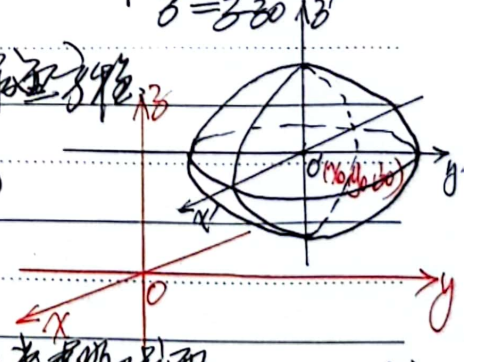
\includegraphics[width=0.3\textwidth]{figure/4-1.png}
    \caption{椭球面}
    \label{fig:椭球面}
\end{figure}

\subsubsection*{圆柱面}

$$
x^2 + y^2 = R^2
$$
为圆柱面,当$z$取任意值时,圆柱面无限延伸.或者说,圆柱面是由直线连续移动形成的,这类曲面称为直纹面.

若要表示$Oxy$平面中的圆$x^2 + y^2 = R^2$,
则应写为$\begin{cases}
    x^2 + y^2 = R^2\\
    z = 0
\end{cases}$,即圆柱面与$Oxy(z=0)$平面的交面.同理,$\begin{cases}
    x^2 + y^2 = R^2\\
    z = 2
\end{cases}$是空间中$z=2$平面上的圆.

\begin{figure}[htbp]
    \centering
    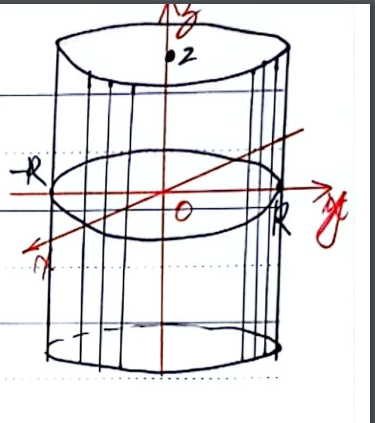
\includegraphics[width=0.3\textwidth]{figure/4-2.png}
    \caption{圆柱面}
    \label{fig:圆柱面}
\end{figure}

\subsubsection*{抛物柱面}

$
y^2 = 2px
$
及$y = a x^2( a , p \neq 0)$为抛物柱面.

$\begin{cases}
    y^2 = 2px\\
    z = 0
\end{cases},\begin{cases}
    y = ax^2\\
    z = 3
\end{cases}$为空间中的抛物线,这称为交面式的抛物线.

\begin{figure}[htbp]
    \centering
    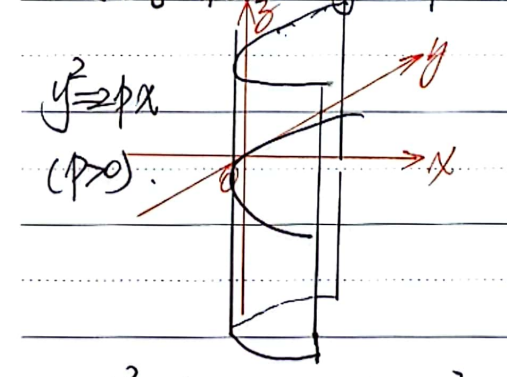
\includegraphics[width=0.3\textwidth]{figure/4-3.png}
    \caption{抛物柱面}
    \label{fig:抛物柱面}
\end{figure}

\subsubsection*{圆锥面}

$$
z^2 = a^2(x^2 + y^2)
$$

而$\begin{cases}
    z^2 = a^2(x^2 + y^2)\\
    z = c
\end{cases}$为空间中的圆;$\begin{cases}
    z = \pm ay\\
    x = 0
\end{cases}$为空间中的相交直线.

\begin{figure}[htbp]
    \centering
    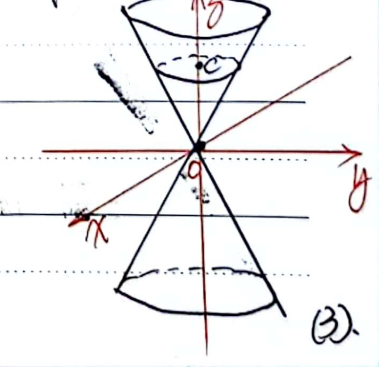
\includegraphics[width=0.3\textwidth]{figure/4-4.png}
    \caption{圆锥面}
    \label{fig:圆锥面}
\end{figure}

\subsubsection*{椭圆抛物面}

$$
z = \frac{x^2}{a^2} + \frac{y^2}{b^2},(a,b > 0)
$$

$\begin{cases}
    z = \frac{x^2}{a^2} + \frac{y^2}{b^2}\\
    z = z_0
\end{cases}$为空间中的椭圆,解$\frac{x^2}{a^2} + \frac{y^2}{b^2} = z_0$可得所围成的面积为$\pi(a\sqrt{z_0})(b\sqrt{z_0}) = \pi abz_0$.

\begin{figure}[htbp]
    \centering
    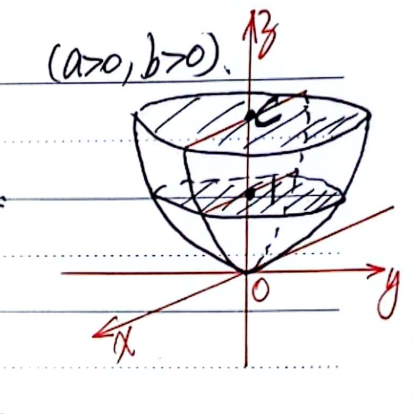
\includegraphics[width=0.3\textwidth]{figure/4-5.png}
    \caption{椭圆抛物面}
    \label{fig:椭圆抛物面}
\end{figure}


\subsubsection*{双曲抛物面}

$$
z = \frac{x^2}{a^2} - \frac{y^2}{b^2},(a,b > 0)
$$

又称为马鞍面.$z = z_0 > 0 $是一族实轴为$x$轴的双曲线,$z = z_0 < 0$是一族虚轴为$y$轴的双曲线.$\begin{cases}
    z = \frac{x^2}{a^2} - \frac{y^2}{b^2}\\
    x = 0
\end{cases}$是抛物线,$\begin{cases}
    z = \frac{x^2}{a^2} - \frac{y^2}{b^2}\\
    y = 0
\end{cases}$也是抛物线.故称双曲抛物面或马鞍面.易证,马鞍面是直纹面.

\begin{figure}[htbp]
    \centering
    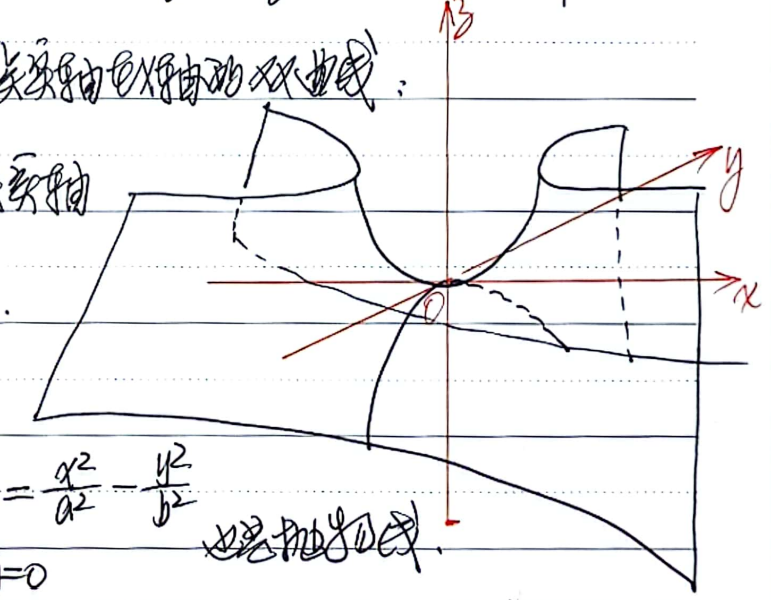
\includegraphics[width=0.3\textwidth]{figure/4-6.png}
    \caption{双曲抛物面}
    \label{fig:双曲抛物面}
\end{figure}

\subsubsection*{双叶双曲面}

$$
\frac{x^2}{a^2} + \frac{y^2}{b^2} - \frac{z^2}{c^2} = -1
$$

从$\frac{x^2}{a^2} + \frac{y^2}{b^2} = \frac{z^2}{c^2} - 1$可知$|z|\ges c$时,才有实点.当$z = z_0 > c$或$z = z_0 < -c$时,都是椭圆.


\begin{figure}[htbp]
    \centering
    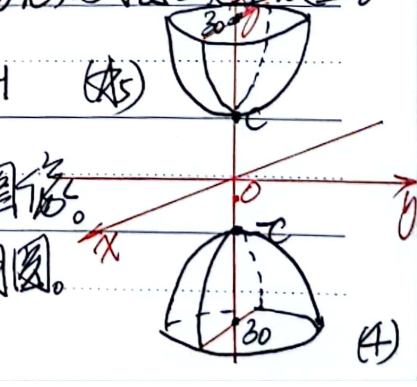
\includegraphics[width=0.3\textwidth]{figure/4-7.png}
    \caption{双叶双曲面}
    \label{fig:双叶双曲面}
\end{figure}

\subsubsection*{单叶双曲面}

$$
\frac{x^2}{a^2} + \frac{y^2}{b^2} - \frac{z^2}{c^2} = 1
$$

从$\frac{x^2}{a^2} + \frac{y^2}{b^2} = \frac{z^2}{c^2} + 1 \ges 0, \forall z$可知,对$z \in \R$,都有曲面图像,任取$z_0 \in \R$,$\begin{cases}
    \frac{x^2}{a^2} + \frac{y^2}{b^2} = \frac{z^2}{c^2} + 1\\
    z = z_0
\end{cases}$都是椭圆,即用垂直于$z$轴的平面去切单叶双曲面,截面都是椭圆.易证,单叶双曲面是由直线连续移动形成的直纹面.

\begin{figure}[htbp]
    \centering
    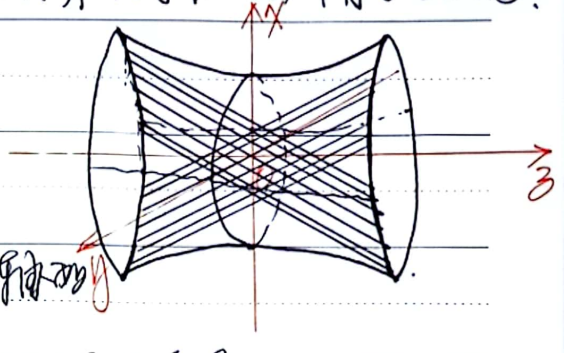
\includegraphics[width=0.3\textwidth]{figure/4-8.png}
    \caption{单叶双曲面}
    \label{fig:单叶双曲面}
\end{figure}

\section{旋转曲面}

设$L:z = f(y)$是一条平面曲线,将$L$绕$Ox$轴旋转一周,则所得曲面称为旋转曲面,记为$\Sigma$.设$M(x,y,z)$是$\Sigma$上一点,过点$M$作$Oz$轴的垂面交$Oz$轴于点$Q(0,0,z)$,交曲线$L$于点$A(0,y_1,z)$,则$| QM|^2 = | QA|^2 \Rightarrow x^2 + y^2 = y_1^2$,即$y_1 = \sqrt{x^2 + y^2}$,所以$\Sigma$的方程为$z = f(\pm \sqrt{x^2 + y^2})$.

\begin{figure}[htbp]
    \centering
    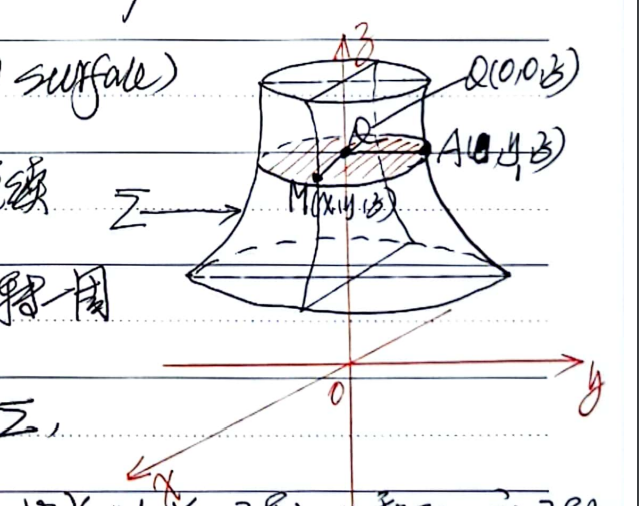
\includegraphics[width=0.3\textwidth]{figure/4-9.png}
    \caption{旋转曲面}
    \label{fig:旋转曲面}
\end{figure}

即曲线$z = f(y)$绕$Ox$轴旋转一周所得旋转曲面中$z$保持不变,而另一个变量用$\pm \sqrt{x^2 + y^2}$代替.同理,曲线$z = f(y)$绕$Oy$轴旋转一周所得旋转曲面中$z$保持不变,而另一个变量用$\pm \sqrt{x^2 + z^2}$代替.

\begin{example}
    证明:
    \begin{enumerate}
        \item 马鞍面:$z = \frac{x^2}{a^2} - \frac{y^2}{b^2}$是直纹面.
        \item 单叶双曲面:$\frac{x^2}{a^2} + \frac{y^2}{b^2} - \frac{z^2}{c^2} = 1$是直纹面.
    \end{enumerate}
\end{example}

\begin{proof}
    

    \begin{enumerate}
        \item 马鞍面可以化为$\left( \frac{x}{a} - \frac{y}{b} \right) \left( \frac{x}{a} + \frac{y}{b} \right) = z$,即$\begin{cases}
        \frac{x}{a} - \frac{y}{b} = \lambda\\
        \frac{x}{a} + \frac{y}{b} = \frac{z}{\lambda}
    \end{cases}$当$\lambda = 0$连续变化时,交面式的直线$L:\begin{cases}
        \frac{x}{a} - \frac{y}{b} = \lambda \\
        \frac{x}{a} + \frac{y}{b} = \frac{z}{\lambda}
    \end{cases}$连续变化,最后形成马鞍面.故马鞍面是直纹面.
        \item 从$\frac{x^2}{a^2} + \frac{y^2}{b^2} = \frac{z^2}{c^2} + 1$可知,对$\left( \frac{y}{b} - \frac{z}{c} \right) \left( \frac{y}{b} + \frac{z}{c} \right) = \left( 1 - \frac{x}{a} \right) \left( 1 + \frac{x}{a} \right)$,因此得到$\begin{cases}
        \frac{y}{b} - \frac{z}{c} = \lambda \left(1 - \frac{x}{a} \right)\\
        \frac{y}{b} + \frac{z}{c} = \frac{1}{\lambda} \left( 1 + \frac{x}{a} \right)
        \end{cases}$当$\lambda = 0$连续变化时,交面式的直线即单叶双曲面是由一族直线连续移动形成的,故单叶双曲面是直纹面.
    \end{enumerate}
\end{proof}


\begin{example}
    \textbf{球面三角形的余弦定理}

    设单位球面三角形$ABC$,是过球心$O$的三个平面$\pi_1,\pi_2,\pi_3$与球面$\Sigma: x^2 + y^2 + z^2 = 1$相交而成的球面上的三角形,如图所示:

    则有
    $$\cos a = \cos b \cos c + \sin b \sin c \cos A$$
    $$\cos b = \cos c \cos a + \sin c \sin a \cos B$$
    $$\cos c = \cos a \cos b + \sin a \sin b \cos C$$
\end{example}

\begin{figure}[htbp]
    \centering
    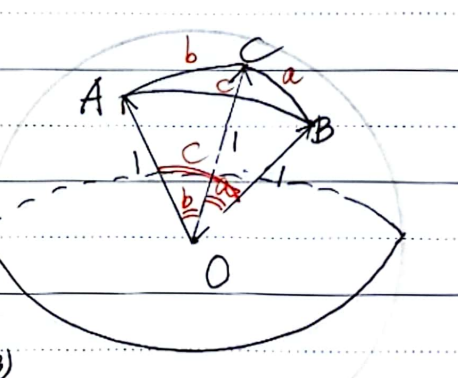
\includegraphics[width=0.5\textwidth]{figure/4-10.png}
    \caption{球面三角形}
    \label{fig:球面三角形}
\end{figure}

\begin{proof}
    $\overrightarrow{OB},\overrightarrow{OC}$确定了平面$\pi_1$,则法向量$\n_1 = \overrightarrow{OB} \times \overrightarrow{OC}$,同理可得$\n_2 = \overrightarrow{OC} \times \overrightarrow{OA},\n_3 = \overrightarrow{OA} \times \overrightarrow{OB}$.

    则
    $$ \cos A = \cos(\n_2,\n_3) = \frac{\n_2 \cdot \n_3}{| \n_2 | | \n_3 |} = \frac{(\overrightarrow{OC} \times \overrightarrow{OA}) \cdot (\overrightarrow{OA} \times \overrightarrow{OB})}{| \overrightarrow{OC} \times \overrightarrow{OA} | | \overrightarrow{OA} \times \overrightarrow{OB} |} $$

    依向量乘法以及Lagrange恒等式,及$| \overrightarrow{OA} \times \overrightarrow{OC} | = | \overrightarrow{OA} | | \overrightarrow{OC} | \sin(\overrightarrow{OA},\overrightarrow{OC}) = \sin b$,$| \overrightarrow{OA} \times \overrightarrow{OB} | = \sin c$,可得$(\overrightarrow{OA} \times \overrightarrow{OC}) \cdot (\overrightarrow{OA} \times \overrightarrow{OB}) = (\overrightarrow{OA} \cdot \overrightarrow{OA})(\overrightarrow{OC} \cdot \overrightarrow{OB}) - (\overrightarrow{OA} \cdot \overrightarrow{OB})(\overrightarrow{OC} \cdot \overrightarrow{OA}) = (| \overrightarrow{OA} |^2 \cos 0 ) (| \overrightarrow{OC}|| \overrightarrow{OB} | \cos a) - (| \overrightarrow{OA} | | \overrightarrow{OB} | \cos b)(| \overrightarrow{OC} | | \overrightarrow{OA} | \cos c) = \cos a - \cos b \cos c$.

    代入,得
    $$\cos A = \frac{\cos a - \cos b \cos c}{\sin b \sin c} \Rightarrow \cos a = \cos b \cos c + \sin b \sin c \cos A$$
    同理可得$\cos b = \cos c \cos a + \sin c \sin a \cos B,\cos c = \cos a \cos b + \sin a \sin b \cos C$.

\end{proof}

\begin{example}
    求曲线$L:\begin{cases}
        \frac{y^2}{a^2} + \frac{z^2}{b^2} = 1\\
        x = 0
    \end{cases}$绕$Oy$轴,$Oz$轴旋转一周所得曲面的方程.

\end{example}

\begin{solution}
\begin{enumerate}
    \item $L$绕$Oy$轴旋转一周,$y$保持不变,$z$用$\pm \sqrt{x^2 + z^2}$代替,则所得曲面方程为
    $\frac{y^2}{a^2} + \frac{x^2 + z^2}{b^2} = 1$,即$\frac{x^2}{b^2} + \frac{y^2}{a^2} + \frac{z^2}{b^2} = 1$.
    \item $L$绕$Oz$轴旋转一周,$z$保持不变,$y$用$\pm \sqrt{x^2 + y^2}$代替,则所得曲面方程为
    $\frac{x^2 + y^2}{a^2} + \frac{z^2}{b^2} = 1$,即$\frac{x^2}{a^2} + \frac{y^2}{a^2} + \frac{z^2}{b^2} = 1$.
\end{enumerate}
\end{solution}

\begin{example}
    求直线$L:\begin{cases}
        y = kx,k \neq 0\\
        z = 0
    \end{cases}$绕$Ox,Oy$轴旋转一周所得曲面的方程.
\end{example}

\begin{solution}
    \begin{enumerate}
        \item 绕$x$轴旋转时,$x$保持不变,$y$用$\pm \sqrt{y^2 + z^2}$代替,则所得曲面方程为
        $y = kx \Rightarrow kx = \pm \sqrt{y^2 + z^2}$,即$k^2x^2 = y^2 + z^2,k \neq 0$.
        \item 绕$y$轴旋转时,$y$保持不变,$x$用$\pm \sqrt{x^2 + z^2}$代替,则所得曲面方程为
        $y = kx \Rightarrow y = k \pm \sqrt{x^2 + z^2}$,即$y^2 = k^2(x^2 + z^2),k \neq 0$.
    \end{enumerate}

    两个旋转曲面都是圆锥面方程.
\end{solution}

\begin{figure}[htbp]
    \centering
    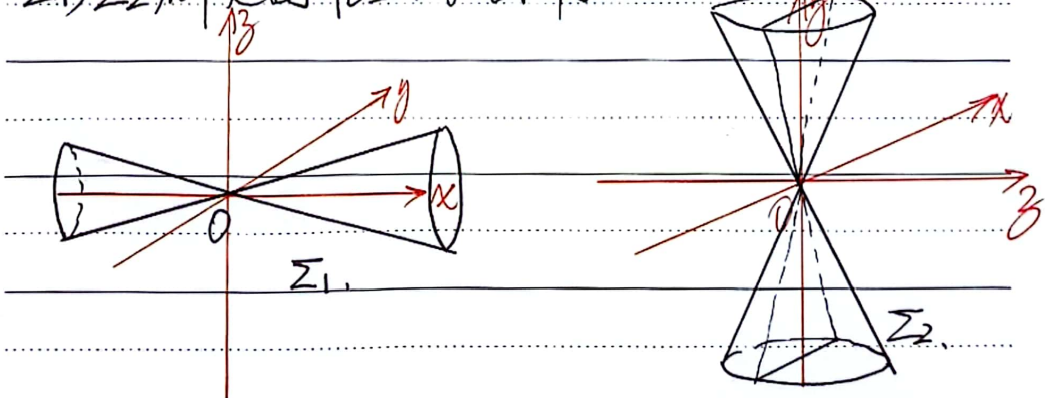
\includegraphics[width=0.8\textwidth]{figure/4-11.png}
    \caption{圆锥面}
    \label{fig:圆锥面}
\end{figure}


\begin{homework}
ex8.3:1,2,3.
\end{homework}







